\documentclass[12pt]{article}
\usepackage{currothesis}
\usepackage[left=1.5in, right=1.5in, top=1in, bottom=1in]{geometry}
\usepackage{fontspec}
%\setmainfont{Adobe Caslon Pro}
\usepackage{layout}
\usepackage[]{amsmath}
\usepackage{amssymb}
\usepackage{ragged2e}
\usepackage{graphicx}
\usepackage{cite}
\usepackage{ mathrsfs }
\usepackage{booktabs}
\usepackage{tikz}
\usepackage{caption}
\captionsetup[table]{skip=10pt}
\usetikzlibrary{matrix,chains,positioning,decorations.pathreplacing,arrows}

\DeclareMathOperator*{\argmin}{arg\,min}

\usepackage{titlesec}

\setcounter{secnumdepth}{4}

\titleformat{\paragraph}
{\normalfont\normalsize\bfseries}{\theparagraph}{1em}{}
\titlespacing*{\paragraph}
{0pt}{3.25ex plus 1ex minus .2ex}{1.5ex plus .2ex}

\def\toclevel@paragraph{4}
\setcounter{tocdepth}{4}
\pagestyle{plain}
\setlength{\marginparwidth}{1in}

\newcommand\tline[2]{$\underset{\text{#1}}{\text{\underline{\hspace{#2}}}}$}

\begin{document}

% Title page
\thispagestyle{empty}
\begin{center}
\Large

THE COOPER UNION\\
ALBERT NERKEN SCHOOL OF ENGINEERING

\vspace{1in}

{
\LARGE
A Deep Partitioned Autoencoder \\for De-Noising Live Audio

}

\vspace{1in}

by

Ethan Lusterman

\vspace*{\fill}

A thesis submitted in partial fulfillment\\
of the requirements for the degree of\\
Master of Engineering

\vspace{1in}

September 2016

\vspace{1in}

Professor Sam Keene, Advisor

\end{center}

% Signature Page
\newpage
\thispagestyle{empty}
\begin{center}
\Large
THE COOPER UNION FOR THE \\ADVANCEMENT OF SCIENCE AND ART

\vspace{0.5in}

ALBERT NERKEN SCHOOL OF ENGINEERING

\vspace{1in}

\justify

This thesis was prepared under the direction of the Candidate's Thesis Advisor
and has received approval. It was submitted to the Dean of the School of
Engineering and the full Faculty, and was approved as partial fulfillment of
the requirements for the degree of Master of Engineering.

\raggedright

\vspace{1in}

\hfill \tline{Dean, School of Engineering \hfill Date}{3in}

\vspace{1in}

\tline{Prof. Sam Keene, Thesis Advisor \hfill Date}{3in}


\end{center}

\newpage
\pagenumbering{roman}
\setcounter{page}{1}

\newpage

\begin{center}
{\Large Acknowledgements} \\

\vspace{1in}
Ack example
\end{center}

\newpage

\begin{center}
{\Large Abstract} \\

\vspace{1in}
Traditional audio denoising systems are often linear time-invariant (LTI) and often require access to clean data to properly train to remove noise. Since clean audio is often unavailable, we build on a partitioned denoising autoencoder for denoising audio signals when clean examples are unavailable for training. In addition, the nonlinearity of a neural network architecture provides additional gains over standard linear models. We compare existing semi-supervised denoising systems as well as canonical supervised denoising autoencoders. We show that for moderate levels of noise, our autoencoder can outperform existing schemes.

\end{center}


\newpage

\tableofcontents

\newpage

\listoffigures

\newpage

Table of Nomenclature

\clearpage
\setcounter{page}{1}
\pagenumbering{arabic}

\fontsize{12pt}{24pt}\selectfont
\section{Introduction}
Advances in smartphone technology have led to smaller devices with more powerful audio hardware, allowing for common consumers to make higher quality recordings. However, recorded speech and music are subject to noisy conditions, often hampering intelligibility and listenability. The goal of denoising audio recordings is to improve intelligibility and perceived quality. A variety of applications of audio denoising exist, including listening to a recording of a band or an artist's live performance in a noisy crowd, or listening to a recorded conversation or speech under noisy conditions.

A common technique for denoising involves the use of autoencoder neural networks. \cite{liu2014experiments} Advances in parallel graphics processing units (GPU) and in machine learning algorithms have allowed for training deeper networks faster, utilizing more hidden layers with more neurons.

Prior work in denoising audio has involved the use of noise-free training data. Since common consumers do not often have access to clean audio, we seek to denoise without the use of clean audio. Other work has touched on such a semi-supervised scenario but was used more as a preprocessing step to a classification algorithm than as time-domain denoising. \cite{stow}

In this thesis, we compare several neural network architectures and problem scenarios, ranging from data input types, level of noise, depth of network, training objectives, and more. In Chapter 2, we present background information on machine learning, neural networks, and signal processing as well as prior work in audio denoising. In Chapter 3, we detail the problem formally as well as introduce our signal model and sourced data. In Chapter 4, we detail all considered network architectures. In Chapter 5, we compare results from different data inputs, levels of noise, network architectures, and training objectives and discuss methods of evaluation. Finally, we make conclusions and recommendations for future work in Chapter 6.

\newpage

\section{Background}
\subsection{Machine Learning}
% explain ML basics
Machine learning involves the use of computer algorithms to make decisions based on training data. Generally, this falls into categorizing input data (classification) or determining a mathetmatical function to determine a continuous output given an input (regression). Popular classification examples include recognizing handwritten digits as well as determining whether an image contains a cat or a dog. An example of a regression problem is determining the temperature given a set of input features (humidity, latitude, longitude, date, etc.).

Problems where training data contain input data vectors as well as the correct output vectors (targets) are known as supervised learning problems. Training a model to denoise audio where noise was introduced to the clean audio would be a supervised learning problem. On the other hand, training a model to denoise audio where the underlying clean signal is not known is an unsupervised learning problem. Different loss (objective) functions and neural network architectures can be exploited to accomplish denoising without the clean data.

For the purposes of this thesis, we use machine learning to determine an underlying nonlinear function that removes noise from time slices of audio (i.e. regression). These slices can then be pieced back together through overlap-add resynthesis. To clarify, this is a general linear model that maps an input noisy audio vector $y[n]=x[n]+N[n]$ to $\tilde{x}[n]$, a target denoised audio vector, where $x[n]$ is the underlying clean signal and $N[n]$ is the additive background noise.

\subsubsection{Regression}
A classical regression technique is linear regression, where one or more independent variables $x_{i}$ are used to determine a scalar dependent variable $y$. The case of a single independent variable $x$ is known as simple linear regression. More formally, for $k$ independent variables, we would like to determine a weight vector $\vec{w}$ and bias vector $\vec{b}$:

\begin{align}
y_i &= w_{1}x_{i1} + \cdots + w_{k}x_{ik} + b_{i}, \qquad i=1\ldots ,n \\
\vec{y} &= \vec{x^T}\vec{w} + \vec{b}
\end{align}

where the rows of $x^{T}$ are the example input observations and $\vec{y}$ and $\vec{b}$ are column vectors.

By extension, the case of linearly estimating a vector output giving a vector input is known as a generalized linear model. A canonical example would be estimating a sine wave $x[n]$ over some number of $N$ samples given noisy samples $y[n]=x[n]+N[n]$.


% \subsubsection{Overfitting and Curse of Dimensionality}


% \subsubsection{Loss functions and Regularization}


% \subsubsection{Gradient Stuff?}


\subsection{Neural Networks}
% Basic explanation of NN
In this thesis, we deal only with feed-forward neural networks, which are essentially directed acyclic graphs (DAG) for computation. In other words, information only moves through the network in one direction.

\subsubsection{Dense Layer}



\subsubsection{Convolutional Layer}



\subsubsection{Nonlinearity Choice}



\subsubsection{Minibatches}



\subsubsection{Batch Normalization}



\subsubsection{Weight Updates}


% \subsubsection{Neural networks as computational graphs}

% A neural network generally is a computational graph $G = (V, E)$ where the
% vertices $V$ correspond to nodes of computation, and the edges $E$ correspond
% to data flow paths connecting the computational nodes. We limit our discussion
% to feed-forward or directed acyclic graphs, in other words graphs where given
% a starting vertex $v$ we are unable to follow the directed edges away from it
% and return to $v$. With this limitation in place we are able to focus on
% stateless graphs, which treat input data examples independently of one another.

% With the additional limitation that all computational nodes in the graph
% perform differentiable operations, and that some nodes are parametric, we are
% able to use automatic differentiation and a gradient descent like optimization
% algorithm to optimize the parameters of the graph against a differentiable
% loss function \cite{DBLP:journals/corr/BaydinPR15}. Automatic differentiation
% is an alternative to numeric and symbolic differentiation, that is efficient,
% accurate to machine precision, and scalable to arbitrary graphs consisting of
% elementary operations. The core tenet of automatic differentiation is that
% since graph vertices are differentiable we can perform the chain rule at each
% node to build up gradients of the full graph. Several machine learning
% frameworks, such as Theano and TensorFlow implement automatic differentiation,
% allowing us to specify the functional form of the graph and getting gradients
% at minimal cost \cite{bergstra-proc-scipy-2010,DBLP:journals/corr/AbadiABBCCCDDDG16}.

% \subsubsection{Fully connected neural networks}
% \label{sec:nn}

% While we have introduced the idea that neural networks can be made up of
% arbitrary computational nodes, there are several common types of nodes that
% are used to build up a toolkit of functional forms at our disposal. First, let
% us a consider a simple inner product with signature:
% \begin{equation}
% \langle \cdot, \cdot \rangle \colon \mathbb{R}^n \times \mathbb{R}^n \to \mathbb{R}
% \end{equation}
% And functional form:
% \begin{equation}
% \langle \mathbf{w}, \mathbf{x} \rangle = \sum\limits_{i = 1}^n w_ix_i
% \end{equation}

% We can interpret this inner product as a single node in our graph, with
% parameters $\mathbf{w}$ and input vector $\mathbf{x}$. While this functional
% form is nice, in that it's linear, and easy to define, it's limited by the
% fact that it brings the rich space $\mathbb{R}^n \times \mathbb{R}^n$ down to
% $\mathbb{R}$ which has limited representational power for problems of interest
% in machine learning. Instead we'll follow a common design pattern, and create
% an array of inner product nodes at a constant number of hops from the source node
% in the graph, or as we'll refer to from here on, at a constant depth. In this case the signature would be:
% \begin{equation}
% g \colon \mathbb{R}^{n \times m} \times \mathbb{R}^n \to \mathbb{R}^m
% \end{equation}
% And functional form:
% \begin{equation}
% g\left(W, \mathbf{x}\right)_j = \sum\limits_{i=1}^n w_{ij}x_i
% \end{equation}
% which we recognize as ordinary matrix multiplication $W\mathbf{x}$, where $W
% \in \mathbb{R}^{n \times m}$. We call this collection of nodes at a common
% depth a layer. This type of matrix multiplication layer is generally referred to
% as a linear, dense, or fully connected layer.

% Layers can be connected together with the goal of creating a more powerful model.
% If we feed one dense layer into another directly we have have a functional form:
% \begin{equation}
% \mathbf{y} = W_n \cdots W_3W_2W_1\mathbf{x}
% \end{equation}

% where the $W_i$'s are all compatible. However this approach is actually
% equivalent to a single matrix multiply $W\mathbf{x}$ where $W$ is the matrix
% product of the $W_i$'s, so we did not actually achieve our goal of higher
% representational power. Our model is still merely linear.

% To address this issue the we introduce the addition of a non-linear
% transformation $f(\cdot)$ (known as an activation function) at the output of
% the matrix multiply. So instead our functional form would be:
% \begin{equation}
% \mathbf{y} = f(W_n \cdots f(W_3f(W_2f(W_1\mathbf{x})))\cdots)
% \end{equation}
% As long as $f(\cdot)$ is differentiable we are able to train our now highly
% non-linear model with our methods of automatic differentiation and gradient
% based optimization.

% Finally we introduce a bias $\mathbf{b}$ so that each node in a layer is not
% constrained to intercept zero. Therefore our full functional form for a single fully
% connected layer with a non-linearity is:
% \begin{equation}
% \mathbf{y} = f\left(W\mathbf{x} + \mathbf{b}\right)
% \label{dense}
% \end{equation}
% with $W \in \mathbb{R}^{n\times m}$ and $\mathbf{b} \in \mathbb{R}^m$.

% A traditional activation function is the sigmoid function:
% \begin{equation}
% S(t) = \frac{1}{1 + e^{-t}}
% \end{equation}

% which maps $t \in \mathbb{R}$ (i.e the interval $[-\infty, \infty]$) to $S(t)$
% on the interval $[0,1]$. This can allow the interpretation of $S(t)$ as a
% probability. Using this activation function Cybenko proved the universal
% approximation theorem \cite{cybenko1989approximation} which shows that neural
% networks of the form in Figure \ref{densenn} can approximate any function with
% appropriate domain and codomains given a large of enough number nodes in the
% middle layer, generally referred to as a hidden layer.

% \begin{figure}
% \begin{center}
% 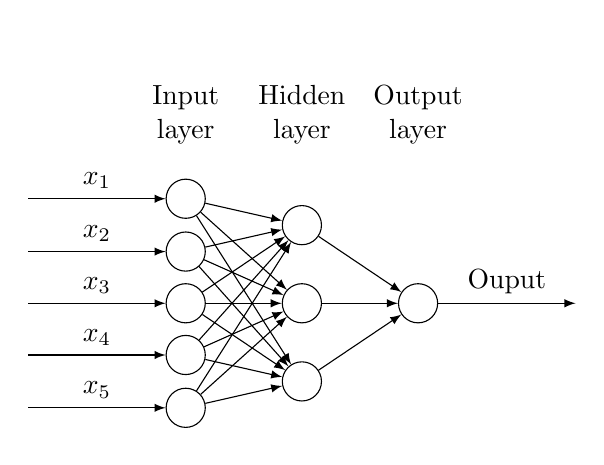
\begin{tikzpicture}[
plain/.style={
  draw=none,
  fill=none,
  },
net/.style={
  matrix of nodes,
  nodes={
    draw,
    circle,
    inner sep=5pt
    },
  nodes in empty cells,
  column sep=-0.5cm,
  row sep=-5pt
  },
>=latex
]
\matrix[net] (mat)
{
|[plain]| \parbox{1.3cm}{\centering Input\\layer} & |[plain]| \parbox{1.3cm}{\centering Hidden\\layer} & |[plain]| \parbox{1.3cm}{\centering Output\\layer} \\
& |[plain]| \\
|[plain]| & \\
& |[plain]| \\
|[plain]| & |[plain]| \\
& & \\
|[plain]| & |[plain]| \\
& |[plain]| \\
|[plain]| & \\
& |[plain]| \\
};
\foreach \ai [count=\mi ]in {2,4,...,10}
  \draw[<-] (mat-\ai-1) -- node[above] {$x_\mi$} +(-2cm,0);
\foreach \ai in {2,4,...,10}
{\foreach \aii in {3,6,9}
  \draw[->] (mat-\ai-1) -- (mat-\aii-2);
}
\foreach \ai in {3,6,9}
  \draw[->] (mat-\ai-2) -- (mat-6-3);
\draw[->] (mat-6-3) -- node[above] {Ouput} +(2cm,0);
\end{tikzpicture}
% \end{center}
% \caption[Feed-forward fully-connected network]{A single hidden layer feed-forward neural network. Each directed
% connection has a scaling factor $w_{ij}$ associated with it; these entries make
% up the $W$ matrix. Each circle, now referred to as a neuron, performs the
% sum and activation functions corresponding to the matrix multiply, and
% mapping by $f(\cdot)$ in Equation \ref{dense}. Layers in the middle of the
% network are referred to as hidden layers because they are not directly observable
% --- instead these are latent variables.}
% \label{densenn}
% \end{figure}

% Figure \ref{densenn} shows a feed-forward network with one hidden-layer. The
% outputs of the hidden layer are referred to as latent variables and are a new type of
% representation for the input data $\mathbf{x}$. With each hidden-layer added to
% the network increasingly complex data representations may be available, but the
% networks will also tend to over-fit their training data as the number of
% parameters increase. In order to combat over-fitting, and increase the
% generalization performance of the network new types of architectures have been
% proposed.


% \subsubsection{Convolutional neural networks}
% % The first convolutional neural network was proposed by Fukushima in 1980 \cite{conv}.
% % The idea of the network is that instead of creating a weight matrix $W$ with
% % parameters that correspond to every entry in $\mathbf{x}$, that there would be a
% % kernel of some small size that would be swept across across $\mathbf{x}$. This
% % process is essentially a convolution. Mathematically this process is:
% % \begin{equation}
% % \mathbf{y} = f(\mathbf{x} \star \mathbf{w})
% % \end{equation}
% % Where $\star$ represents a discrete convolution, $\mathbf{w}$ is a
% % one-dimensional kernel and $f(\cdot)$ is an activation function. This method can
% % be extended to work for two and three-dimensional data representations, for
% % example:
% % \begin{equation}
% % Y = f(X \star W)
% % \end{equation}
% % where $Y,X$ and $W$ are all matrices.
% \subsubsection{Convolutions with holes}
% \subsubsection{Tranposed convolutions}
% \subsubsection{Additional techniques}
% \paragraph{Dropout}
% Various teams have demonstrated that in deep networks neurons can learn
% complex co-adaptation schemes; that is deep neurons respond to ``mistakes'' in
% shallower neurons. In order to prevent co-adaptation, so that each neuron
% learns a meaningful representation, the dropout scheme has been proposed
% \cite{JMLR:v15:srivastava14a,DBLP:journals/corr/abs-1207-0580,dahl2013improving}.
% Dropout is a masking process. In order to apply dropout to a layer during
% training, a binary mask is applied across neurons. The mask is determined by
% sampling a Bernoulli distribution with a parameter $p$ corresponding to the
% probability that a neuron will be masked. When a neuron is masked its output
% is considered fixed at zero. When the network is used for evaluation no masks
% are applied and all neurons are connected.
% \paragraph{Batch normalization}
% \paragraph{Rectified linear units}
% Various activations have been proposed on the basis of similarity to the
% potential activations in actual biological neurons in human eyes. Recently the
% rectified linear unit (ReLU) has demonstrated significant performance
% increases for network generalization and increased training speed
% \cite{glorot2011deep,dahl2013improving}. The ReLU activation is defined as
% $\text{max}(0,x)$. In other words a ReLU activation forwards along any
% positive inputs and sets and negative inputs to zero.
% \paragraph{Exponential linear units}
% \paragraph{Residual networks}
% \paragraph{Minibatch training}
% Traditionally there were two different approaches to optimizing neural
% network parameters, the online approach and the batch approach. In the online
% approach, the parameters of the network are updated after each exposure to a
% training example and gradient calculation. In the batch approach, the network
% is exposed to all of the training examples, the gradients are accumulated and
% then the network's parameters are updated. This was long believed to be the
% better approach, as the accumulated and averaged gradient was more likely to
% be an estimate of the ``true'' gradient of the network towards an optimized
% solution. It was later shown  that, while the batch mode may give a better
% estimate of the gradient, due to the noise and its stochastic nature, the
% online approach actually leads to a faster convergence time, in terms of
% number of examples \cite{Wilson:2003:GIB:965268.965272}. This is because in
% the stochastic approach the optimizer is less likely to get stuck in local
% minima. An alternative approach that recently has become popular is the mini-
% batch approach. In this approach some number of examples, say $N$, are exposed
% to the network, the gradients are accumulated, and the parameters are updated.
% In this case $N$ is much less than the total number of training examples
% available. This approach, with serial computational resources really only
% represents a decrease in training speed, because it is fairly similar to the
% batch approach. The reason this approach has become popular lately is that
% with the parallel resources afforded by modern high performance graphics
% processing units (GPUs) the increase in example-wise training time becomes a
% decrease in wall-time to train.

% \paragraph{Intelligent parameter initialization}
% Kaiming et al. have demonstrated an improved parameter initialization
% technique specifically designed for neurons with ReLU activations
% \cite{DBLP:journals/corr/HeZR015}. This approach derives a method that enables
% extremely deep models comprised of ReLU neurons to converge rather than stall,
% as they would with other initialization schemes. The initial parameters for
% the convolutional layers are drawn from a zero mean normal distribution with a
% standard deviation of  $\sqrt{2/n_l}$. Where $n_l = k^2c$. This corresponds to
% the number of connections in the response for $k\times k$ kernels processing
% $c$ input channels.

% \paragraph{ADAM optimizer}
% \paragraph{Style loss}

\subsection{Signals and Systems}
Domain knowledge of discrete audio signals and systems better informs our decisions for an audio denoising system, so some background information on signals and systems as it pertains to this thesis is detailed below.

\subsubsection{Signals}
We deal exclusively with discrete-time audio signals in this thesis. A discrete-time audio signal $x[n]$ is represented as a sequence of numbers (samples), where each integer-valued slot $n$ in the sequence corresponds to a unit of time based on the sampling frequency $f_s$. This comes from sampling the continuous-time audio signal $x_c(t)$:
\begin{equation}
x[n] = x_c(nT)
\end{equation}

where $T=1/f_s$.
For example, a 1-second speech signal sampled at 8kHz has 8000 samples. Furthermore, digital signals also have discrete valued sample amplitudes. For the purposes of this thesis, the bit depths of computers we use for analysis are high enough to allow for perfect reconstruction between continuous-time signals and digital signals.

We also assume signals collected have been properly sampled according to the Nyquist-Shannon sampling theorem, which states that a discrete-time signal must be sampled at at least twice the highest frequency present in the signal to prevent aliasing of different frequencies. For example, speech signals genearlly have information up to 8kHz, so many speech signals are sampled at 16kHz. Music is more complex in that signals often span up to about 20kHz, so CD quality recordings are often sampled at 44.1kHz or higher. For this thesis, we use recordings sampled at 44.1kHz or lower.


\subsubsection{Convolution}
The discrete-time convolution operation takes two sequences $x[n]$ and $h[n]$ and outputs a third sequence $y[n] = x[n] * h[n]$:

\begin{equation}
y[n] = \sum_{k=-\infty}^{\infty} x[k]h[n-k]
\end{equation}

A linear, time-invariant (LTI) system is characterized by its impulse response $h[n]$, which allows us to determine samples $y[n]$ when $x[n]$ is subject to $h[n]$. For the purposes of this thesis, our underlying clean signal $x[n]$ might be subject to the conditions of an acoustic environment $h[n]$ and crowd noise $N[n]$:
\begin{equation}
y[n] = h[n]*x[n]+N[n]
\end{equation}

In this scenario, our system would attempt to recover $h[n]*x[n]$ and possibly $x[n]$ if the acoustic environment were deemed ``noisy enough.''

One of our proposed systems also incorporates convolutional neural networks (CNN), which use convolutions between samples instead of simple linear combinations (discussed later).

\subsubsection{Frequency Transforms}



\subsubsection{Windowing and Perfect Reconstruction}

\newpage

\section{System Description}
\newpage


\section{Results}
We present results here for mainly shallow network architectures. At the output layer of each network, an identity nonlinearity is used. At any other layer, the modified ReLU (mReLU) is used. Unless otherwise noted, batch normalization is applied at the input layer. Each network is compared first to itself at varying noise levels (-6 dB, -3 dB, 0 dB, 3 dB, 6 dB SNR) in terms of convergence as well as the mean squared error (MSE) for inferences.

Training minibatches consist of 128 examples, each with 1024-sample FFT frames of $\norm{Y[k]}$ at a sampling rate 16 kHz. Time windows are windowed using the Hanning window, and we use 50\% overlap for perfect reconstruction at inference time. The examples used are a sum of sine waves at four fixed frequencies with uniform random amplitude and phase. The frequencies are chosen to form an A4 major chord (1-3-5-8) at slightly de-tuned frequencies so as not to allow the network to learn any pattern from the immediate harmonic structure.

\begin{align}
f &= [441, 549, 660, 881]\qquad \text{Hz}\\
x[n] &= \sum_{i=0}^{3} A_i \sin{2 \pi f_i / f_s n + \phi_i}, \qquad n=0\ldots ,1023\\
A_i &\sim U(0.25, 0.75)\\
\phi &\sim U(0, 2\pi)
\end{align}

Applied noise is additive-white Gaussian noise (AWGN), with the variance $\sigma^2$ selected to achieve the desired average SNR for each minibatch as in Equation \ref{eq:siggy}.

\begin{align}
N[n] &\sim N(0, \sigma^2), \qquad n=0\ldots ,1023\\
y[n] &= x[n] + N[n]
\end{align}

In semi-supervised cases where we use the soft label $y$ for noise-only versus signal-plus-noise examples, we use 25\% noise-only examples per minibatch. For inference calculations, we construct a minibatch with consecutive overlapping, windowed frames.

Simulations are written in Python 2.7 using Lasasgne \cite{sander_dieleman_2015_27878}, a ``lightweight library to build and train neural networks in Theano.'' Theano is a ``Python library that allows you to define, optimize, and evaluate mathematical expressions involving multi-dimensional arrays efficiently.'' \cite{2016arXiv160502688short} Theano boasts parallel GPU support, numpy support (a mathematical Python library), numerical stability, and symbolic differentiation, among other features. These libraries and frameworks allow for ease of developing deep, novel architectures and save time in doing things like calculating gradients, weight updates and back-propagation. Sample simulation code is shown in the Appendix.

Weight updates are calculated using Adam updates \cite{DBLP:journals/corr/KingmaB14}. 2000 iterations (minibatches) are used for each simulation. Unless otherwise noted, each hidden layer uses 2000 hidden nodes.

\subsection{Supervised Autoencoder}

For the following results, we show

\subsubsection{Batch Normalized Input}

\begin{figure}[!ht]
\centering
\includegraphics[width=.8\textwidth]{../thesis/thesis/comparisons/plotfinal/pdf/paris-loss}
\caption{Loss at various SNRs for Supervised Single-Layer Autoencoder with Batch Normalization at the Input}
\end{figure}

\begin{figure}[!ht]
\centering
\includegraphics[width=.8\textwidth]{../thesis/thesis/comparisons/plotfinal/pdf/paris-mse}
\caption{MSE at various SNRs for Supervised Single-Layer Autoencoder with Batch Normalization at the Input}
\end{figure}

\subsubsection{Non-Batch Normalized Input}

\begin{figure}[!ht]
\centering
\includegraphics[width=.8\textwidth]{../thesis/thesis/comparisons/plotfinal/pdf/paris-nobatchnorm-loss}
\caption{Loss at various SNRs for Supervised Single-Layer Autoencoder without Batch Normalization at the Input}
\end{figure}

\begin{figure}[!ht]
\centering
\includegraphics[width=.8\textwidth]{../thesis/thesis/comparisons/plotfinal/pdf/paris-nobatchnorm-mse}
\caption{MSE at various SNRs for Supervised Single-Layer Autoencoder with Batch Normalization at the Input}
\end{figure}


\subsection{Partitioned Autoencoder}

\begin{figure}[!ht]
\centering
\includegraphics[width=.8\textwidth]{../thesis/thesis/comparisons/plotfinal/pdf/dan-dense-loss}
\caption{Loss at various SNRs for Single-Layer Partitioned Autoencoder\cite{stow}}
\end{figure}

\begin{figure}[!ht]
\centering
\includegraphics[width=.8\textwidth]{../thesis/thesis/comparisons/plotfinal/pdf/dan-dense-mse}
\caption{MSE at various SNRs for Single-Layer Partitioned Autoencoder\cite{stow}}
\end{figure}

\subsection{Partitioned Curro Autoencoder}

\begin{figure}[!ht]
\centering
\includegraphics[width=.8\textwidth]{../thesis/thesis/comparisons/plotfinal/pdf/curro-loss}
\caption{Loss at various SNRs for Single-Layer Curro Autoencoder}
\end{figure}

\begin{figure}[!ht]
\centering
\includegraphics[width=.8\textwidth]{../thesis/thesis/comparisons/plotfinal/pdf/curro-mse}
\caption{MSE at various SNRs for Single-Layer Curro Autoencoder}
\end{figure}

\subsection{Comparison of Loss Convergence}

\begin{figure}[!ht]
\centering
\includegraphics[width=.8\textwidth]{../thesis/thesis/comparisons/plotfinal/pdf/comparison-loss--6}
\caption{Loss Comparison of Various Networks at -6 dB}
\end{figure}

\begin{figure}[!ht]
\centering
\includegraphics[width=.8\textwidth]{../thesis/thesis/comparisons/plotfinal/pdf/comparison-loss--3}
\caption{Loss Comparison of Various Networks at -3 dB}
\end{figure}

\begin{figure}[!ht]
\centering
\includegraphics[width=.8\textwidth]{../thesis/thesis/comparisons/plotfinal/pdf/comparison-loss-0}
\caption{Loss Comparison of Various Networks at 0 dB}
\end{figure}

\begin{figure}[!ht]
\centering
\includegraphics[width=.8\textwidth]{../thesis/thesis/comparisons/plotfinal/pdf/comparison-loss-3}
\caption{Loss Comparison of Various Networks at 3 dB}
\end{figure}

\begin{figure}[!ht]
\centering
\includegraphics[width=.8\textwidth]{../thesis/thesis/comparisons/plotfinal/pdf/comparison-loss-6}
\caption{Loss Comparison of Various Networks at 6 dB}
\end{figure}



\subsection{Comparison of Mean Squared Error Convergence}

\begin{figure}[!ht]
\centering
\includegraphics[width=.8\textwidth]{../thesis/thesis/comparisons/plotfinal/pdf/comparison-mse--6}
\caption{MSE Comparison of Networks at -6 dB}
\end{figure}

\begin{figure}[!ht]
\centering
\includegraphics[width=.8\textwidth]{../thesis/thesis/comparisons/plotfinal/pdf/comparison-mse--3}
\caption{MSE Comparison of Networks at -3 dB}
\end{figure}

\begin{figure}[!ht]
\centering
\includegraphics[width=.8\textwidth]{../thesis/thesis/comparisons/plotfinal/pdf/comparison-mse-0}
\caption{MSE Comparison of Networks at 0 dB}
\end{figure}

\begin{figure}[!ht]
\centering
\includegraphics[width=.8\textwidth]{../thesis/thesis/comparisons/plotfinal/pdf/comparison-mse-3}
\caption{MSE Comparison of Networks at 3 dB}
\end{figure}

\begin{figure}[!ht]
\centering
\includegraphics[width=.8\textwidth]{../thesis/thesis/comparisons/plotfinal/pdf/comparison-mse-6}
\caption{MSE Comparison of Networks at 6 dB}
\end{figure}


\newpage


\section{Conclusions and Future Work}
\subsection{Conclusions}
While more work is needed, deep partitioned neural network architectures using time and frequency data seem promising in long-term solutions for denoising speech and music signals.

\subsection{Future Work}
\subsubsection{Models}
Make network deeper. Consider gradual partitioning instead of hard.

\subsubsection{Data}
Get more data. Consider different noise levels and types of signals.


\newpage

\nocite{*}
\fontsize{12pt}{16pt}\selectfont
\bibliography{bib}{}
\bibliographystyle{IEEEtran}

\end{document}
